\documentclass[a11paper]{article}

\usepackage{karnaugh-map}
\usepackage{subcaption}
\usepackage{tabularx}
\usepackage{titlepage}
\usepackage{document}
\usepackage{booktabs}
\usepackage{multicol}
\usepackage{float}
\usepackage{varwidth}
\usepackage{graphicx}
\usepackage{siunitx}
% \usepackage[toc,page]{appendix}
\usepackage[usenames,dvipsnames]{xcolor}

\title{Rapport d'APP}

\class{Logique Combinatoire}
\classnb{GEN420 \& GEN430}

\teacher{Marwan Besrour \& Gabriel Bélanger}

\author{
  \addtolength{\tabcolsep}{-0.4em}
  \begin{tabular}{rcl} % Ajouter des auteurs au besoin
      Benjamin Chausse & -- & CHAB1704 \\
      Shawn Couture    & -- & COUS1912 \\
  \end{tabular}
}

\newcommand{\todo}[1]{\begin{color}{Red}\textbf{TODO:} #1\end{color}}
\newcommand{\note}[1]{\begin{color}{Orange}\textbf{NOTE:} #1\end{color}}
\newcommand{\fixme}[1]{\begin{color}{Fuchsia}\textbf{FIXME:} #1\end{color}}
\newcommand{\question}[1]{\begin{color}{ForestGreen}\textbf{QUESTION:} #1\end{color}}

\begin{document}
\maketitle
\newpage
\tableofcontents
\newpage

\section{Module \texttt{thermo2bin}}
\subsection{Démarche et équations}

L’objectif était de convertir un code thermométrique de 12 bits en un code
binaire non signé sur 4 bits. Le nombre représenté par un tel code est obtenu
en comptant le nombre de bits à 1. Les équations logiques doivent donc
effectuer ce comptage. Étant donné que le code est sur 12 bits, il a été
divisé en trois groupes de 4 bits, ce qui a permis l'utilisation de tables de
Karnaugh pour déterminer les équations logiques.

D'après la table de vérité du code thermométrique 4 bits
(\ref{tab:table-de-vérité-thermométrique-4-bits}), le bit le plus
significatif du résultat binaire n’est jamais à 1. L'équation du bit $E$ est
donc simplement $E = 0$. Le bit $F$ est à 1 uniquement si $A$ l’est
également, d’où l’équation $F = A$. Les tables de Karnaugh ont donc été
utilisées uniquement pour les deux bits restants. Les deux tables, une pour
chaque bit, se trouvent en annexe (\ref{tab:karnaugh-bit-G} et
\ref{tab:karnaugh-bit-H}). Les équations étant assez simple, aucune simplification d'équations était nécessaire.

\begin{align}
	E & = 0         \\
	F & = A         \\
	G & = A'C       \\
	H & = C'D + A'B
\end{align}

Les trois résultats binaires sont ensuite additionnés à l’aide d’un
additionneur 4 bits, afin d’obtenir la valeur totale correspondant au nombre
de bits à 1 dans le code thermométrique. En ce qui concerne la détection
d'erreurs, une vérification par groupe de 2 bits est effectuée. Celle-ci
s’assure que, pour chaque paire consécutive, le LSB n’est pas à 0 si le MSB
est à 1, ce qui permet une détection rapide d’erreurs éventuelles (voir le
code en annexe).

\subsection{Explication des schémas blocs}

Le module \texttt{thermo2bin} est constitué de deux additionneurs 4 bits,
chacun composé de quatre additionneurs 1 bit. Les additionneurs 1 bit ont été
implémentés à l’aide de logique combinatoire ainsi que de blocs utilisant des
instructions \texttt{case}. Le module thermométrique comprend trois sections
identiques effectuant la conversion d’un code thermométrique 4 bits en un
code binaire non signé. Il intègre également une section de détection
d’erreurs, qui agit directement sur l’entrée du module. Il est à noter que
Vivado optimise certains sous-modules à l’aide de tables de correspondance
(\textit{look-up tables}) afin d’améliorer leur performance par rapport à une
implémentation reposant uniquement sur des portes logiques élémentaires.

\subsection{Fréquence d’opération}

Pour déterminer la fréquence d’opération maximale, il faut analyser le schéma
obtenu lorsque tout les sous-modules sont combinés et identifier le chemin le
plus long qu’un signal peut parcourir de l’entrée à la sortie. Cette analyse
peut être effectuée en observant les schémas générés par Vivado.

Le chemin le plus long à l’intérieur d’un additionneur 1 bit se situe entre
les bits d’entrée et le signal de retenue (\textit{carry-out}), ce qui
représente un total de 3 portes logiques dans le premier additionneur 1 bit.
Par la suite, les additionneurs 1 bit sont chaînés via les signaux
\textit{carry-in} et \textit{carry-out}, avec 2 portes logiques
supplémentaires par liaison. Un additionneur 4 bits utilise ainsi 4
additionneurs 1 bit en série, ce qui donne un chemin critique de
$2 \times 4 + 1 = 9$ portes logiques.

Le module \texttt{thermo2bin} contient deux additionneurs 4 bits chaînés. Le
second additionneur reçoit en entrée le \textit{carry-out} du premier,
ajoutant 8 portes logiques supplémentaires. Le total pour les deux blocs est
donc d’environ 17 portes logiques. Du côté des entrées, le bit le plus
coûteux en logique est $H$, avec le chemin suivant : $C' \rightarrow (C'D)
	\rightarrow (C'D + A'B)$, soit 3 portes logiques supplémentaires. On obtient
ainsi un total d’environ 20 portes logiques.

En supposant un temps de propagation de $5,\text{ns}$ par porte, le temps de
propagation maximal est donc approximativement $20 \times 5 = 100,\text{ns}$.
Sans tenir compte du temps de lecture ni des \textit{buffers} que Vivado
pourrait ajouter aux entrées et sorties, la fréquence maximale estimée est :

\begin{align}
	\frac{1}{100 \times 10^{-9}} & \approx \SI{10}{\mega\hertz}
\end{align}

Ce résultat est loin des $20,\text{MHz}$ exigés. Cependant, Vivado optimise
les additionneurs 1 bit à l’aide de \textit{look-up tables}, réduisant le
circuit logique de 3 à 1 porte logique dans certains cas. Cela abaisse le
nombre total de portes logiques à environ 11, ce qui améliore la fréquence
maximale à:

\begin{align}
	\frac{1}{11 \times 5 \times 10^{-9}} & \approx \SI{18.18}{\mega\hertz}
\end{align}

Ce n’est toujours pas suffisant pour atteindre l’objectif fixé.

\subsection{Implémentation}

Le code VHDL du module \texttt{thermo2bin} est fourni en annexe. Trois
composantes sont utilisées de façon hiérarchique. Le module principal aurait
pu être divisé en sous-modules de 4 bits, mais pour des raisons
d’optimisation, les trois conversions de segments de 4 bits du vecteur
thermométrique de 12 bits sont intégrées dans un seul bloc.

Après l’instruction \texttt{begin}, on retrouve trois sections quasi
identiques effectuant les équations booléennes de conversion. Les résultats
sont stockés dans trois signaux intermédiaires, lesquels sont additionnés
séquentiellement à l’aide d’additionneurs 4 bits. Le résultat du premier et
du deuxième segment est additionné, puis le résultat est additionné au
troisième segment. Un signal de retenue (\textit{carry}) permet la liaison
entre les deux additionneurs. Le résultat final est assigné à la sortie du
module \texttt{thermo2bin}. La logique de détection d’erreur est placée à la
fin du code et a été expliquée dans la section sur la démarche.

Le code VHDL de l’additionneur 4 bits est simple : quatre instances de
l’additionneur 1 bit y sont instanciées. Des signaux intermédiaires assurent
la propagation du \textit{carry} d’un bloc à l’autre ainsi que la
transmission des bits à additionner à chaque position. Le premier
additionneur traite les bits de poids faible (\textit{LSB}) et transmet le
\textit{carry} au suivant, qui additionne les bits de poids 1, et ainsi de
suite.

Les additionneurs 1 bit sont eux aussi simples : ils sont issus d’une table
de vérité à partir de laquelle une expression booléenne a été dérivée.

\section{Simulation Complète}
Tout les modules du projet ont leurs propre test bench avec leurs tests unitaire. Par conséquent, le testbench de AppCombiTop n'a pas
tout les tests de 7 segments. Il test que les boutons changent les deux DELs de parité et que l'entrée ADCth change les DELs PMOD.
Le testbench de Thermo2bin test tout les cas de figure valide et quelques tests invalide. Les autres testbench testent les modules
individuellement pour tout les cas de figure ou presque tout. Il était donc redondant et trop long de refaire tout ces tests unitaire la
dans le test bench d'AppCombiTop, car une duplication des fonctionalitées testé aurait lieux.
\\
Le banc de test du Mux ne tests pas toutes les possibilitées. Étant donnée qu'il est composé de 3 autres composantes lesquels ont leurs
propre banc de tests, cela aurait créé des tests redondant. Il test les combinaisons de boutons donnant une erreur,
s'assure que celle-ci est envoyé aux 7 segments, que l'erreur en entrée fonctionne, et que toutes combinaisons de boutons valide affiche
les bon nombre sur les 7 segments en sortie. Il test aussi la présence du Moin 5 sur la sortie signée.
\\
Le test de thermo2bin n'a pas besoin de tester les $2^{12}$ possibilité. Il suffit de tester les $12$ valide puis de tester que la
détection d'erreur fonctionne sur toutes les paires de $2$ bits. Ensuite, quelques tests avec plusieurs zéros aléatoire sont effectué
juste pour confirmé.
\\
Les banc de tests utilisent des "assert" qui permet d'afficher dans le terminal si des problèmes ont eut lieux (résultat obtenu diffère
du résultat voulu). La plus part fonctionne parfaitement tandis que d'autre montre quelques problèmes liés aux "undefined" qui causent des
affichage d'erreur incohérent tel que: "Obtenu 0 Voulu 0". Malgrès beaucoup de deboggage et le fonctionnement réelle du module, le banc de
test du Mux montre des problème de changements et est difficile à lire. Le numéro de test est donc fournis dans son chronogramme. Pour le
banc de test de parité, deux chronogrammes sont fournis en fonction de l'état du bouton (cfg). Les banc de tests démontres quelques
problèmes de valeurs initiales, comme une valeur de sortie qui change alors que l'entrée n'a pas changé. L'approche utilisé pour faire
les bancs de tests devra être révisé afin de mitiger ces problèmes de chronogrammes. Tout les banc de tests ont des "expected" pour les
"outputs" attendu. Leurs noms sont directement en lien avec la fonctionalité du module et pas forcément le nom du signal haut niveau.

\section{Démarche d'analyse de compatibilité}
La première étape à été d'analyser le signal d'entrée de la carte thermométrique. La DEL 2 est connecté au connecteur JD1 en
configuration "pull-up". Ceci dit, il faut donc avoir un 0 logique à son entrée pour l'allumé. Cependant, trois inverseurs sont
connecté en série avant elle. Soit deux 74V1T04STR et un NC7SP04P5X alimenté à +1.2 Volts. Après analyse de $V_{OH}$, $V_{OL}$, $V_{IL}$
et $V_{IH}$ des deux portes logiques, le NC7SP04P5X à un $V_{OH}$ de maximum 1.1 volts tandis que le 74V1T04STR à besoin d'un $V_{IH}$
minimum de 2 Volts. Donc selon le 74V1T04STR, le NC7SP04P5X envoie toujours un niveau logique bas, ce qui résulte à une del
tout le temps allumé sauf lorsque le connecteur de test de la del est en mode de test car un bon niveau logique haut est envoyé à
l'entrée des 74V1T04STR.

\newpage
\appendix
\section{Code VHDL}
\todo{Finish this this}

\begin{figure}[H]
	\tiny
	\centering
	\begin{varwidth}{\linewidth}
		\begin{verbatim}
architecture Behavioral of Thermo2Bin is
    signal first_segment_of_four : STD_LOGIC_VECTOR(3 downto 0);
    signal second_segment_of_four : STD_LOGIC_VECTOR(3 downto 0);
    signal third_segment_of_four : STD_LOGIC_VECTOR(3 downto 0);

    component Add4Bits is
        Port ( A : in STD_LOGIC_VECTOR (3 downto 0);
            B : in STD_LOGIC_VECTOR (3 downto 0);
            C : in STD_LOGIC;
            R : out STD_LOGIC_VECTOR (3 downto 0);
            Rc : out STD_LOGIC);
    end component;

    signal first_plus_second : STD_LOGIC_VECTOR(3 downto 0);
    signal carry_out_first_plus_second : STD_LOGIC;
    signal last_carry_out : STD_LOGIC;

begin
    first_segment_of_four(3) <= '0';
    first_segment_of_four(2) <= thermo_bus(11);
    first_segment_of_four(1) <= NOT thermo_bus(11) AND thermo_bus(9);
    first_segment_of_four(0) <= NOT thermo_bus(11) AND ((NOT thermo_bus(9) AND thermo_bus(8)) OR (thermo_bus(10) AND thermo_bus(9)));

    second_segment_of_four(3) <= '0';
    second_segment_of_four(2) <= thermo_bus(7);
    second_segment_of_four(1) <= NOT thermo_bus(7) AND thermo_bus(5);
    second_segment_of_four(0) <= NOT thermo_bus(7) AND ((NOT thermo_bus(5) AND thermo_bus(4)) OR (thermo_bus(6) AND thermo_bus(5)));

    third_segment_of_four(3) <= '0';
    third_segment_of_four(2) <= thermo_bus(3);
    third_segment_of_four(1) <= NOT thermo_bus(3) AND thermo_bus(1);
    third_segment_of_four(0) <= NOT thermo_bus(3) AND ((NOT thermo_bus(1) AND thermo_bus(0)) OR (thermo_bus(2) AND thermo_bus(1)));

    first_plus_second_adder : Add4Bits port map (
      A => first_segment_of_four,
      B => second_segment_of_four,
      R => first_plus_second,
      Rc => carry_out_first_plus_second,
      C => '0');

    plus_third_adder : Add4Bits port map (
      A => first_plus_second,
      B => third_segment_of_four,
      R => binary_out,
      Rc => last_carry_out,
      C => carry_out_first_plus_second);

    error <= (
    (thermo_bus(11) AND NOT thermo_bus(10)) OR
    (thermo_bus(10) AND NOT thermo_bus(9)) OR
    (thermo_bus(9)  AND NOT thermo_bus(8)) OR
    (thermo_bus(8)  AND NOT thermo_bus(7)) OR
    (thermo_bus(7)  AND NOT thermo_bus(6)) OR
    (thermo_bus(6)  AND NOT thermo_bus(5)) OR
    (thermo_bus(5)  AND NOT thermo_bus(4)) OR
    (thermo_bus(4)  AND NOT thermo_bus(3)) OR
    (thermo_bus(3)  AND NOT thermo_bus(2)) OR
    (thermo_bus(2)  AND NOT thermo_bus(1)) OR
    (thermo_bus(1)  AND NOT thermo_bus(0)));

end Behavioral;
\end{verbatim}

	\end{varwidth}
	\caption{Module Thermo2bin}
\end{figure}

\begin{figure}[H]
	\tiny
	\centering
	\begin{varwidth}{\linewidth}
		\begin{verbatim}
architecture Behavioral of Add4Bits is

  signal bufA : STD_LOGIC;
  signal bufB : STD_LOGIC;
  signal bufC : STD_LOGIC;

  component Add1BitA is Port (
    X : in STD_LOGIC;
    Y : in STD_LOGIC;
    Ci: in STD_LOGIC;
    O : out STD_LOGIC;
    Co: out STD_LOGIC);
  end component;

  component Add1BitB is Port (
    X : in STD_LOGIC;
    Y : in STD_LOGIC;
    Ci: in STD_LOGIC;
    O : out STD_LOGIC;
    Co: out STD_LOGIC);
  end component;

begin

  first : Add1BitB port map (
    X  => A(0),
    Y  => B(0),
    Ci => C,
    O => R(0),
    Co => bufA);

  sec : Add1BitB port map (
    X  => A(1),
    Y  => B(1),
    Ci => bufA,
    O => R(1),
    Co => bufB);

  third : Add1BitA port map (
    X  => A(2),
    Y  => B(2),
    Ci => bufB,
    O => R(2),
    Co => bufC);

  fourth : Add1BitA port map (
    X  => A(3),
    Y  => B(3),
    Ci => bufC,
    O => R(3),
    Co => Rc);

end Behavioral;
\end{verbatim}

	\end{varwidth}
	\caption{Module Add4Bits}
\end{figure}

\begin{figure}[H]
	\tiny
	\centering
	\begin{varwidth}{\linewidth}
		\begin{verbatim}
architecture Behavioral of Add1BitA is

begin

  O  <= (X xor Y) xor Ci;
  Co <= ((X xor Y) and Ci) or (X and Y);

end;
\end{verbatim}

	\end{varwidth}
	\caption{Module Add1BitA}
\end{figure}

\begin{figure}[H]
	\tiny
	\centering
	\begin{varwidth}{\linewidth}
		\begin{verbatim}
architecture Behavioral of Add1BitB is

begin

Adder: process(X, Y, Ci) is variable buf: STD_LOGIC_VECTOR(2 downto 0);
begin
  buf(0) := X;
  buf(1) := Y;
  buf(2) := Ci;

  case (buf) is
    when "000" =>
      O  <= '0';
      Co <= '0';
    when "001" =>
      O  <= '1';
      Co <= '0';
    when "010" =>
      O  <= '1';
      Co <= '0';
    when "011" =>
      O  <= '0';
      Co <= '1';
    when "100" =>
      O  <= '1';
      Co <= '0';
    when "101" =>
      O  <= '0';
      Co <= '1';
    when "110" =>
      O  <= '0';
      Co <= '1';
    when "111" =>
      O  <= '1';
      Co <= '1';
    when others =>
      O  <= '0';
      Co <= '0';
  end case;

end process Adder;

end Behavioral;
\end{verbatim}

	\end{varwidth}
	\caption{Module Add1BitB}
\end{figure}

\section{Schémas Bloc}

\todo{Simulations}


\begin{figure}[H]
	\centering
	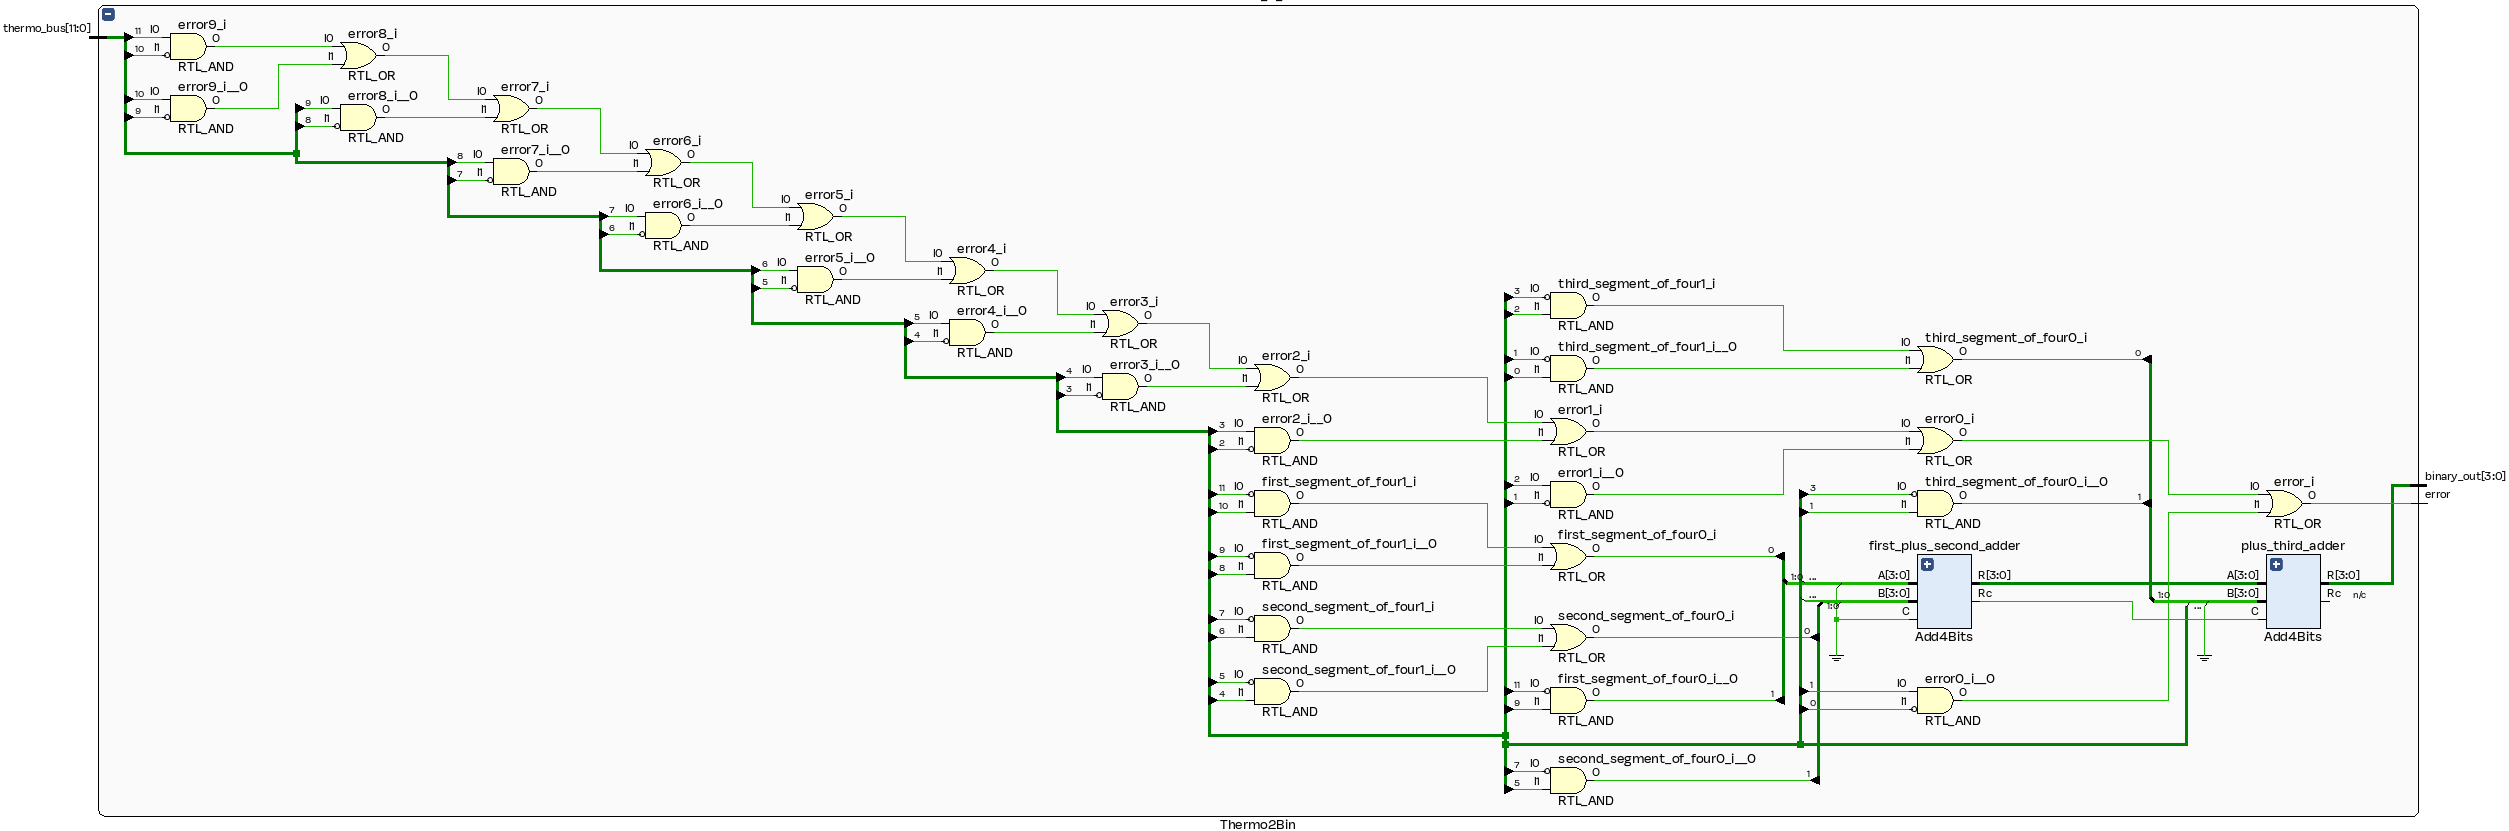
\includegraphics[width=\textwidth]{assets/img/schematic-thermo2bin.png}
	\caption{Module Thermo2bin}
\end{figure}

\begin{figure}[H]
	\centering
	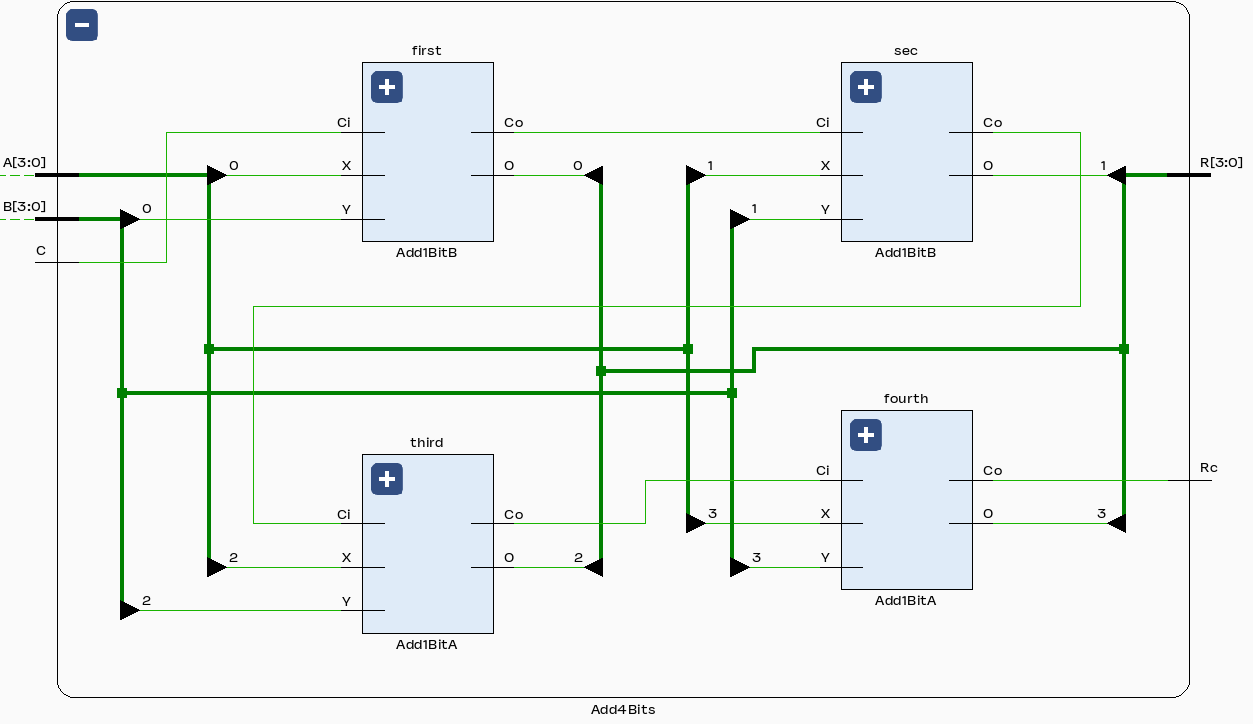
\includegraphics[width=.6\textwidth]{assets/img/schematic-add4bits.png}
	\caption{Module Add4Bits}
\end{figure}

\begin{figure}[H]
	\centering
	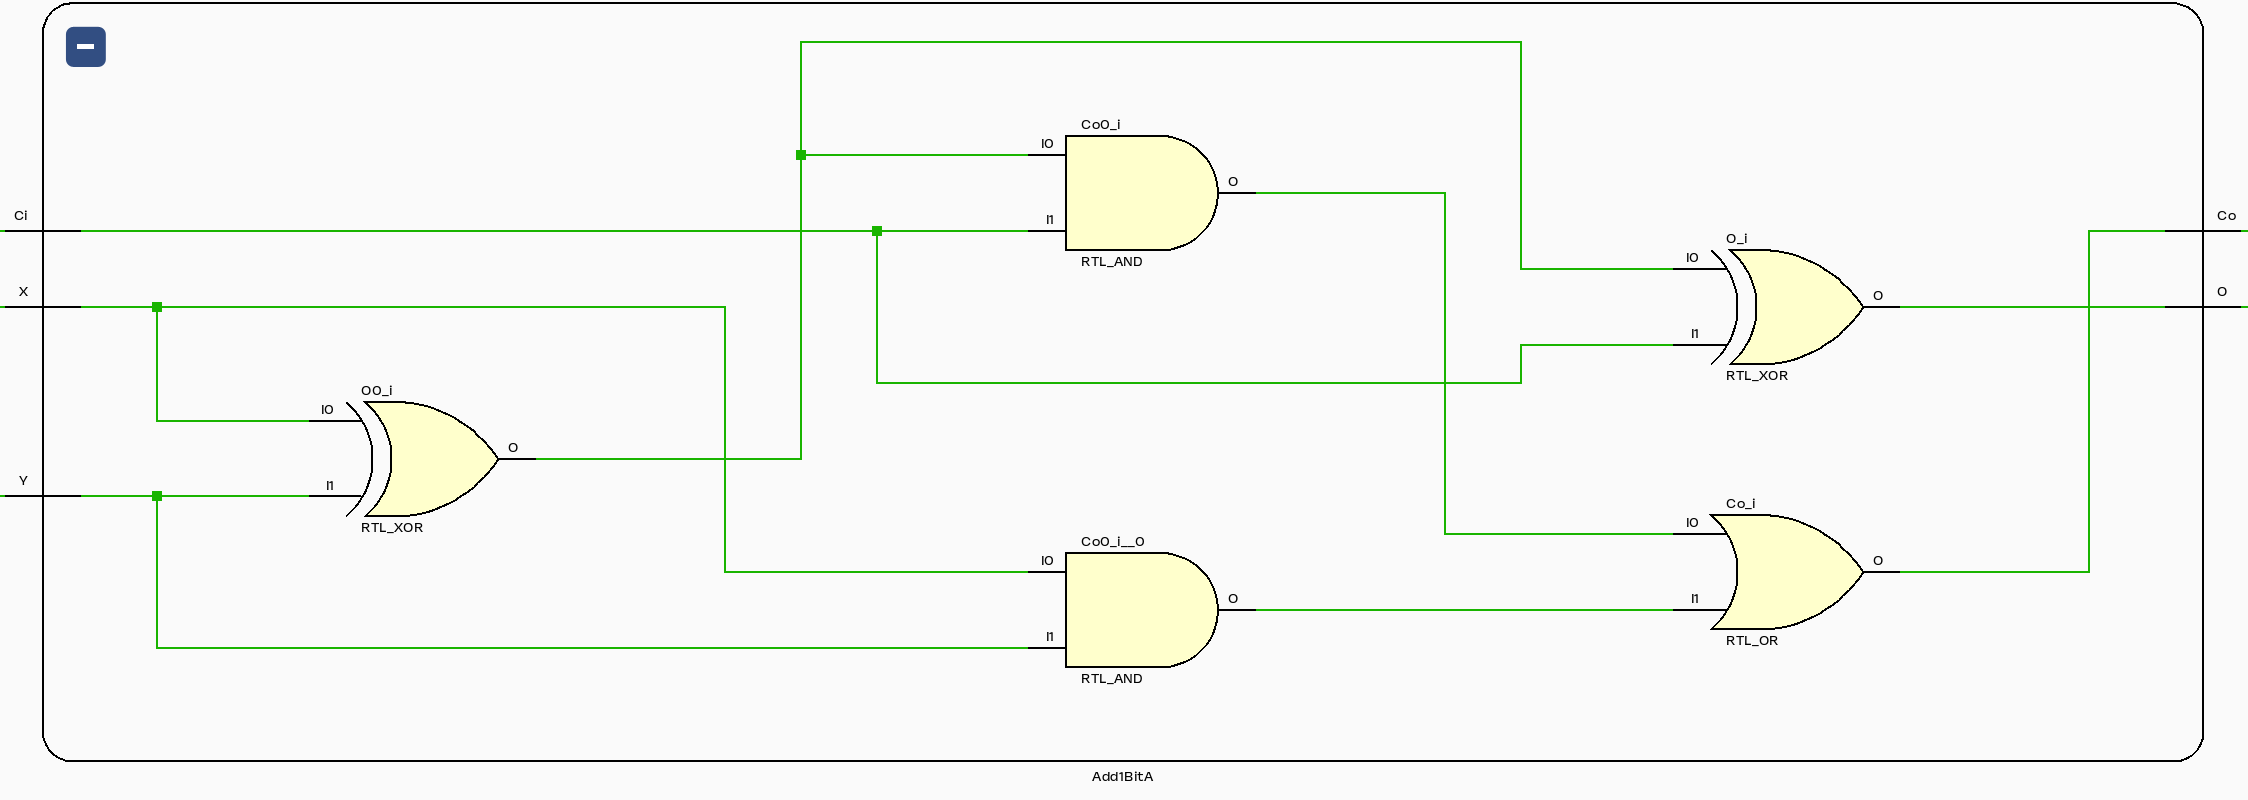
\includegraphics[width=.6\textwidth]{assets/img/schematic-add1bita.png}
	\caption{Module Add1BitA}
\end{figure}

\begin{figure}[H]
	\centering
	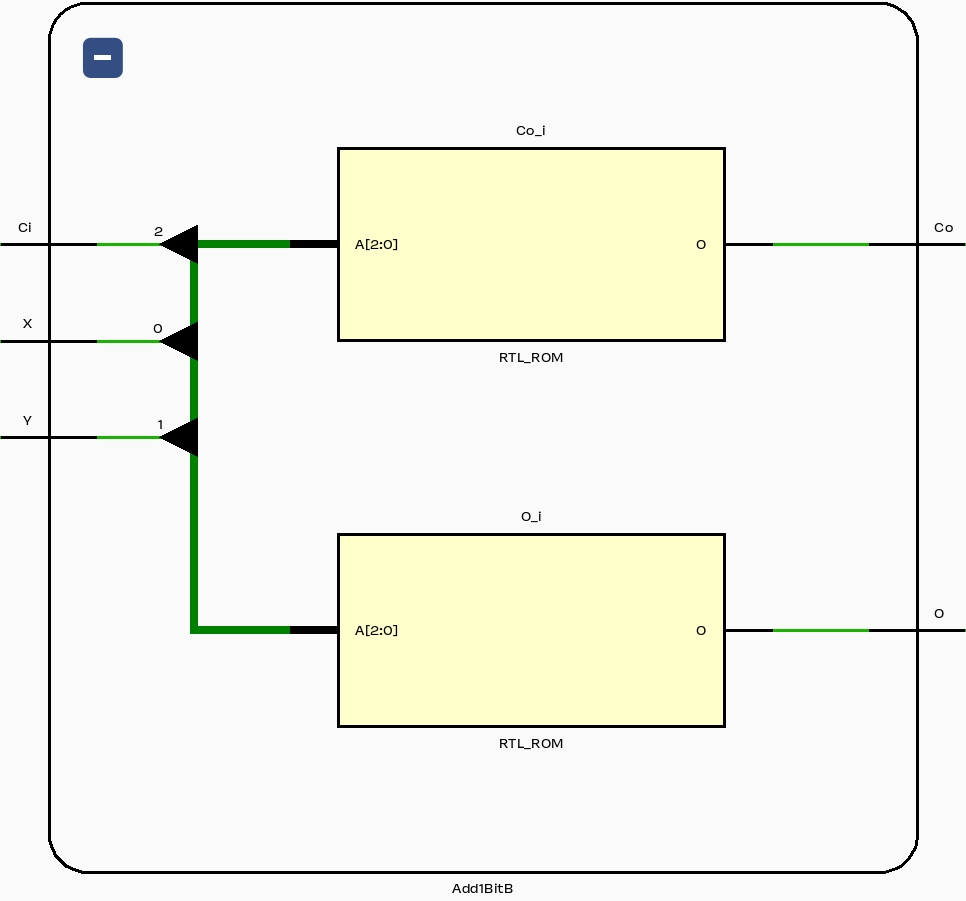
\includegraphics[width=.6\textwidth]{assets/img/schematic-add1bitb.png}
	\caption{Module Add1BitB}
\end{figure}


\newpage
\section{Tables de Vérité et Karnaugh}

% \begin{figure}[H]
% \centering
% \begin{karnaugh-map}[4][4][1][$D$][$C$][$B$][$A$]
% \manualterms{
% 	0,1,2,3,
% 	4,5,6,7,
% 	8,9,10,11,
% 	12,13,14,15}
% \implicant{2}{10}
% \implicant{4}{13}
% \implicant{12}{10}
% \implicantedge{3}{2}{11}{10}
% \end{karnaugh-map}
% \caption{TEMPLATE NOT GOOD}
% \end{figure}


\begin{table}[H]
	\centering
	\caption{Table de vérité des Bits}
	\label{tab:table-de-vérité-thermométrique-4-bits}
	\vspace{.2cm}
	\begin{tabular}{llllllll}
		\toprule
		A & B & C & D & E & F & G & H \\
		\midrule
		0 & 0 & 0 & 0 & 0 & 0 & 0 & 0 \\
		0 & 0 & 0 & 1 & 0 & 0 & 0 & 1 \\
		0 & 0 & 1 & 1 & 0 & 0 & 1 & 0 \\
		0 & 1 & 1 & 1 & 0 & 0 & 1 & 1 \\
		1 & 1 & 1 & 1 & 0 & 1 & 0 & 0 \\
		\bottomrule
	\end{tabular}

\end{table}

\begin{figure}[H]
\centering
\begin{karnaugh-map}[4][4][1][$D$][$C$][$B$][$A$]
\manualterms{
	0,1,X,0,
	X,X,X,1,
	X,X,X,X,
	X,X,X,0}
\implicant{1}{9}
\implicant{4}{6}
\end{karnaugh-map}
\caption{Karnaugh pour le bit $H$}
\label{tab:karnaugh-bit-H}
\end{figure}

\begin{figure}[H]
\centering
\begin{karnaugh-map}[4][4][1][$D$][$C$][$B$][$A$]
\manualterms{
	0,0,X,1,
	X,X,X,1,
	X,X,X,X,
	X,X,X,0}
\implicant{3}{6}
\end{karnaugh-map}
\caption{Karnaugh pour le bit $G$}
\label{tab:karnaugh-bit-G}
\end{figure}

\end{document}
